\documentclass{article}

\usepackage[margin=2cm]{geometry}

\usepackage{amsmath}
\usepackage{amsfonts}
%\usepackage{braket}
\usepackage{tabularx}
\usepackage{amsthm}
\usepackage[braket, qm]{qcircuit}
\usepackage[bookmarks = true, pdfpagemode = None, pdfstartview = FitH, colorlinks = true, urlcolor = blue]{hyperref}
\usepackage{listings}
\usepackage{caption}
\usepackage{subcaption}
\usepackage{graphicx}
\usepackage{algorithm}
\usepackage{placeins}
%\usepackage{algorithmic}
\usepackage[noend]{algpseudocode}
\makeatletter
% Reinsert missing \algbackskip
\def\algbackskip{\hskip-\ALG@thistlm}
\makeatother
\renewcommand{\arraystretch}{1.5}

\theoremstyle{definition}
\newtheorem{definition}{Definition}[section]

\theoremstyle{problem}
\newtheorem{problem}{Problem}[section]

\theoremstyle{lemma}
\newtheorem{lemma}{Lemma}[section]

\title{PhD Project First Year Report\\Optimal Designs for Fault-Tolerant Quantum Computers}
\author{Author: Luke Heyfron\\Supervisor: Dr. Earl T. Campbell}
\date{June 2017}

\begin{document}
	\captionsetup{width=0.8\linewidth}
	\maketitle
	
	\begin{abstract}
		In order to realise practical quantum computation, it is important to consider the resource cost associated with implementing quantum circuits. The T gate requires several hundred times more elementary operations than Clifford group operators to implement fault-tolerantly for certain high-threshold quantum error correction codes such as the surface code. Therefore, effective methods for minimizing the number of T gates in a given quantum circuit are instrumental in reducing the overall cost of quantum computation. Finding the minimum number of T gates required to implement an n-qubit circuit generated by CNOT and T has been shown to be equivalent to minimum distance decoding of the punctured Reed-Muller code of length n and order n-4, which is believed to be a hard problem. In this report, we present two computationally efficient heuristics for estimating the
		minimal number of T gates required for multi-qubit circuits generated by CNOT and T gates. Both algorithms output circuits with T counts that have asymptotic scaling $\mathcal{O}(n^2)$, which is the same scaling as the upper bound for the inefficient optimal decoder and improves upon the worst-case scaling of $\mathcal{O}(n^3)$ for a naive fast decoder. The algorithms can be adapted for circuits over the universal $\{H,CNOT,T\}$ gate set by allowing for ancilla preparation and classical feedforward, and they have been used to estimate the T count for known practical quantum circuits.
	\end{abstract}
	
	\section{Introduction}
	%Certain high threshold quantum error correction codes such as the toric code have transversal implementations of quantum logic gates that generate the logical Clifford group.
	%However, the Clifford group in isolation is insufficient for universal quantum computation: one quantum gate outside the Clifford group must be included in the gate set.
	%This is often chosen to be the T gate, which unfortunately does not have a transversal implementation on the toric code.
	%A standard way to apply a T gate fault-tolerantly to a logically encoded qubit is to prepare a high-fidelity ancillary T-type magic state using magic state distillation protocols, then apply a teleportation gadget between the ancilla and the target qubit. This method involves many more elementary gates than the transversal Clifford gates, which motivates the cost model for logical quantum gates where the Clifford gates are ``free" and T gates are ``expensive". Consequentially, it is of interest to find ways to reduce the number of T gates used in implementations of quantum circuits.
	
	%In order to realise fault-tolerant universal quantum computation, it is important to consider the resources required in implementing quantum circuits.
	For many types of quantum error correction code including the surface code, a special class of so-called Clifford operations have \emph{transversal} implementations \cite{38_Dennis_2001}, meaning the physical gates used to implement a logical operator act independently on each qubit with the same code block \cite{30_Gottesman_1997}. A transversal operator is natively protected by the error correction code against noise and the number of physical gates required for its implementation are linear in the number of physical qubits. Therefore, such operators are assumed to be cheap, perfect resources. However, Clifford operations alone are insufficient for universal quantum computation. The T gate is the common choice for the canonical non-Clifford gate, whose inclusion in the gate set allows for universal quantum computation. The T gate is not transversal for the surface code as well as many other codes and requires many more steps to implement fault-tolerantly. An established method for implementing a T gate requires the distillation of many noisy resource states called magic states into few high-fidelity states over several rounds \cite{32_Bravyi_2005},\cite{33_Bravyi_2012}. The state can then be teleported into a circuit using a scheme such as \cite{39_Gottesman_1999}. The distillation and teleportation stages can be performed with physical Clifford operations but involve many more physical Clifford operations than those of logical Cliffords, which means T gates are considered as high costing gates compared to Clifford operations.
	Therefore, it is of interest to develop protocols for synthesizing quantum circuit decompositions that minimize the number of T gates used.% synthesizing T gate optimal quantum circuits.%optimize quantum circuits with respect to the number of T gates.% develop ways to synthesize circuits that use a minimal number of the T gates. %understand how best we can optimize quantum circuits with respect to the number of T gates.
	
	%Previous work in this area.
	Much work has already been done to develop T gate optimization algorithms. Algorithms for optimizing the T depth, another resource metric for T gates, were developed by Amy, Maslov, Mosca and Roetteler in \cite{3_Amy_2013} and by Amy, Maslov and Mosca in \cite{4_Amy_2013}. Gosset, Kliuchnikov, Mosca and Russo developed an algorithm that finds T count optimal decompositions for multi-qubit Clifford and T circuits \cite{5_Gosset_2013}.
	More recently, Amy and Mosca \cite{8_Amy_2016} proved a relationship between the problem of finding T gate minimal decompositions of circuits composed of CNOT and T gates and minimum distance decoding of the punctured Reed-Muller code of length $n$ and order $n-4$. This was followed by Campbell and Howards work \cite{1_Campbell_2017}, in which a method for simultaneously performing gate synthesis and magic state distillation was proposed that features a fast Reed-Muller decoder based on Lempel's matrix factoring algorithm with improved T count scaling compared to \cite{8_Amy_2016} (see sections \ref{s_Lempel} and \ref{s_rand}).
	
	In this report an algorithm is presented for reducing the T count for $n$-qubit quantum circuits composed of CNOT and T gates. It is shown how it is possible to generalize this algorithm for the universal gate set $\{H, CNOT, T\}$. The rest of the paper is structured as follows: in section \ref{s2_Theory} we define the terminology and notation conventions used for the rest of the paper; in section \ref{s3_Problem} we define the gate synthesis problem that our algorithm solves, first in the quantum circuit picture, then in terms of a special kind of matrix representation that facilitates the description of our solution. In section \ref{s4_Solution} we describe the algorithm presented in this paper for reducing the T count; in section \ref{s5_Results} we present the results of this algorithm compared to previous works for both randomized circuits over CNOT and T as well as practical circuits of a universal gate set. Finally, we consolidate our results and discuss future work in section \ref{s6_Discussion}.
	
	\FloatBarrier
	\section{Theory and Terminology}
	\label{s2_Theory}
		\subsection{Quantum Theory}
		We define the set of $n$-qubit computational basis states to be $\{\ket{x}\}$ for all $x \in \{0,1\}^n$, the set of binary tuples of length $n$.		
		The single qubit Pauli operators are defined in the computational basis as follows,
		\begin{equation}
		\label{e1_Paulis}
		\begin{matrix}
		\sigma_0 = \begin{pmatrix}1 & 0 \\ 0 & 1\end{pmatrix} & \sigma_x = \begin{pmatrix}0 & 1 \\ 1 & 0\end{pmatrix} \\
		& \\
		\sigma_y = \begin{pmatrix}0 & -i \\ i & 0\end{pmatrix} & \sigma_z = \begin{pmatrix}1 & 0 \\ 0 & -1\end{pmatrix}.
		\end{matrix}
		\end{equation}
		The $n$-qubit Pauli group $\mathcal{P}^n$ is defined as the $n$-fold tensor product of single qubit Pauli operators, along with multiplicative factors of $\pm1$ and $\pm i$ i.e. $\mathcal{P}^n = \{\left(-1\right)^a i^b \sigma_c \mid a,b \in \{0,1\}, c \in\{0,x,y,z\}\}^n$.	
		The operators CNOT, H and T are given by
		\begin{equation}
		\label{e2_CNOT}
		\text{CNOT} = \begin{pmatrix}
		1 & 0 & 0 & 0 \\
		0 & 1 & 0 & 0 \\
		0 & 0 & 0 & 1 \\
		0 & 0 & 1 & 0
		\end{pmatrix},
		\end{equation}
		\begin{equation}
		\label{e3_H}
		H = \frac{1}{\sqrt{2}}\begin{pmatrix}
		1 & 1 \\
		1 & -1
		\end{pmatrix},
		\end{equation}
		\begin{equation}
		\label{e4_T}
		T = \begin{pmatrix}
		1 & 0 \\
		0 & \omega
		\end{pmatrix},
		\end{equation}
		where we define $\omega=e^{i\frac{\pi}{4}}$. A single qubit operator $G$ applied to the $i^\text{th}$ qubit of an $n$-qubit system is expressed as $G^{\left(i\right)}$. A controlled-$G$ operator where $G$ is a single qubit target operator is expressed as $\text{control-}G^{\left(t,c\right)}$ where the $t^\text{th}$ and $c^\text{th}$ qubits are the target and control qubit, respectively.
		
		The $n$-qubit Clifford group $\mathcal{C}^n$ is defined as the set of operators that maps $\mathcal{P}^n$ to itself under conjugation, $\mathcal{C}^n = \{U \mid UPU^\dagger = P^\prime, P, P^\prime \in \mathcal{P}^n\}$. The $k^{\text{th}}$ level of the Clifford hierarchy on $n$-qubits, $\mathcal{C}_k^n$, is defined recursively,
		\begin{equation}
		\mathcal{C}_k^n = \{U \mid UPU^\dagger = Q, P \in \mathcal{P}^n, Q \in \mathcal{C}_{k-1}^n\},
		\end{equation}
		with $\mathcal{C}_1^n = \mathcal{P}^n$. We define $\mathcal{D}_k^n \subseteq \mathcal{C}_k^n$ as the set of diagonal elements of the $k^{\text{th}}$ level of the Clifford hierarchy.
		
		%\subsection{Classical Coding Theory}
		
		%\subsection{Reed-Muller Codes}
		
		%\subsection{Notes}
		%NOTE: use mathbf for all matrices and vectors
	
	\FloatBarrier
	\section{The Gate Synthesis Problem}
	\label{s3_Problem}
	%NOTES from Earl's paper:
	%	- magic states model formalized by Bravyi and Kitaev
	%	- Clifford operations are natively protected against noise in many error correcting codes including 2D topological codes such surface codes and 2D color codes.
	%	- Clifford operations: preparation of |0> states, measurement of Pauli group operators, Clifford group operators (normalizer of Pauli group), classical feed forward, access to classical random number generator.
	%	- Non-Clifford operations aren't natively protected so are costly.
	%	- Magic state distillation required (multiple layers) each of which involves many Clifford operations. Therefore, cost of non-clifford operations is significantly more than clifford operations
	%	- We measure resources by counting the number of logical T gates used in a circuit.
	%	- Using Campbell and Howard's synthillation protocol, the circuits can be implemented fault tolerantly with low overhead.
	
	An $n$-qubit quantum circuit $C$ of length $k$ is a time-ordered set of operators taken from an elementary gate set $G$ on $n$ qubits. In particular, if $C$ is such a quantum circuit, then $C = \{C_1,C_2,...,C_k\}$ where $C_t\in G^n$ is the operator applied at the $t^\text{th}$ time step.
	$C$ is said to implement the unitary $U_C$, which is given by
	\begin{equation}
	U_C = \prod_{t = k}^1 C_t.
	\end{equation}
	Two circuits are said to be equivalent if they implement the same unitary, i.e. $C \equiv_U C^\prime$ if $U_C = U_{C^\prime}$. We define $E(g)$ to be the cost function of applying a particular gate $g\in G$ to a logical qubit. The total cost of a circuit is therefore,
	\begin{equation}
	\label{e_Cost}
	E(C) = \sum_{t=1}^k E(C_t).
	\end{equation}
	
	
	
	\theoremstyle{problem}
	\begin{problem}{Gate Synthesis Problem (version 1).}
		\label{p_gsp1}
		Given a unitary $U$, find some circuit $C$ such that $E(C) = \text{min}\{E(C^\prime) \mid \forall C^\prime,U=U_{C^\prime}\}$.
	\end{problem}
	
	According to our cost model for quantum gates, $E(\text{Clifford}) = 0$ and $E(T)=1$. The total cost function for a circuit $C$ is therefore,
	\begin{equation}
	E(C) = \sum_{t=1}^k E(C_t) = \tau(C),
	\end{equation}
	where we define the T count of a circuit, $\tau(C)$, to be the number of T gates in circuit $C$. Therefore, the gate synthesis problem is equivalent to minimizing the number of T gates. We define the T count of a unitary as follows.
	
	\theoremstyle{definition}
	\begin{definition}{\emph{T count.}}
		Given a unitary $U$, the T count is defined as $\tau(U) = \text{min}\{\tau(C) \mid \forall C, U = U_C\}$
	\end{definition}
	
	\FloatBarrier
		\subsection{Circuits Composed of CNOT and T Gates}
	In this section we establish the notions of phase polynomials and gate synthesis matrices following the analyses of \cite{8_Amy_2016} and \cite{1_Campbell_2017}.
	It is known that any unitary $U$ generated by the CNOT and T gate can be decomposed as,
	\begin{equation}
	U = VW,
	\end{equation}
	where $V$ is a member of the Clifford group with $\tau(V)=0$ and $W \in \mathcal{D}_3^n$. It follows that $\tau(W) = \tau(U)$. Due to $V$ not contributing to the T count of $U$, we will assume that $U$ is already diagonal to simplify the analysis.	
	The action of a unitary $U \in \mathcal{D}_3^n$ on a computational basis state can be written as follows,
	\begin{equation}
	U\ket{x} = \omega^{f_U(x)}\ket{x},
	\end{equation}
	where $f_U(x)$ is known as the \emph{phase function} for $U$. The phase function can be determined by tracking the state of each qubit through the circuit, updating appropriately after each CNOT gate, and adding a term after each T gate. See figure \ref{f_phase} for an example. This construction leads to the following decomposition for phase function known as the \emph{phase polynomial},
	\begin{equation}
	f_U(x) = \sum_{y\in\{0,1\}^n\backslash 0} \mathbf{a}_y \bigoplus_{i=1}^n x_i^{y_i}\mod 8,
	\end{equation}
	where $\mathbf{a}\in \mathbb{Z}_8^{2^n}$ is called an \emph{implementation vector}. Modulo 8 arithmetic is due to $\omega$ being the eight root of unity. Once an implementation vector for $U$ is found, it is possible to construct a circuit $C$ that implements $U$ using $\tau(C) = |\mathbf{a} \pmod{2}|$ T gates. There exist multiple implementation vectors that give rise to the same phase functions. This is due to the existence of non-trivial implementation vectors that implement the all-zero phase function. We denote the set of all implementation vectors that implement the all-zero phase function as $\mathcal{R}$. In \cite{8_Amy_2016}, Amy and Mosca proved that the set $\mathcal{R}^\prime = \{r \pmod{2} \mid r \in \mathcal{R}\}$ is exactly the punctured Reed-Muller code of length $n$ and order $n-4$, denoted $RM^*(n-4,n)$.
	
	
	
	%\theoremstyle{definition}
	%\begin{definition}{Gate Synthesis Matrix.}
	%	Let $\mathbf{a}$ be an implementation vector for a phase function $f(x)$. A gate synthesis matrix is an $n\times m$ matrix, $A$, whose elements $A_{i,j} \in GF(2)$, where for each $y$ satisfying $(\mathbf{a}_{y} \mod 2)=1$, there is one column in $A$ such that $A_{i,j}=y_i$ for some $j \in \left[1,m\right]$.
	%\end{definition}

	We now define the gate synthesis matrix, which is central to the description of the algorithms presented in this report.
	\theoremstyle{definition}
	\begin{definition}{\emph{Gate Synthesis Matrix}.}
		Let $f_U(x)$ be a phase function for a unitary $U$. A gate synthesis matrix is a matrix, $A$, whose elements $A_{i,j} \in GF(2)$, that satisfies $f_{(CUC^\prime)}(x) = |A^Tx|$ where $C,C^\prime \in \mathcal{C}_2^n$.
	\end{definition}
	It should be noted that the number of columns of a gate synthesis matrix is equal to $|\mathbf{a} \pmod{2}|$, where $\mathbf{a}$ is the implementation vector for which $A$ is a gate synthesis matrix, and therefore is also equal to the T count of the circuit. This means we can rewrite problem \ref{p_gsp1},
	\theoremstyle{problem}
	\begin{problem}{Gate Synthesis Problem (version 2).}
		Given a unitary $U$, find a gate synthesis matrix $A$ such that $\text{cols}(A) = \text{min}\{cols(A^\prime) \mid \forall A^\prime, f_U(x) = |A^{\prime T}x|\}$, where $cols(A)$ is the number of columns of matrix $A$.
	\end{problem}

	%Note from the definition of a gate synthesis matrix, $m = |\mathbf{a} \mod 2|$, and that any two gate synthesis matrices that differ only by column permutations should be considered equivalent.

	% Put an example here: Circuit -> phase polynomial -> Gate synthesis matrix

	% Phase polynomial
	\begin{figure}[h]
		\[
		\Qcircuit @C=1em @R=0.7em {
			\lstick{\ket{x_1}} & \gate{T} & \ctrl{1} & \qw & \qw & \ctrl{1} & \qw & \qw \\
			& & & \push{\rule{2em}{0em}} & & & & \rstick{\omega^{f(x)}\ket{x_1,x_2}} \\
			\lstick{\ket{x_2}} & \gate{T} & \targ \qwx & \ustick{x_1 \oplus x_2}\qw  & \gate{T} & \targ \qwx & \ustick{x_2}\qw  & \qw
		}
		\]
		\caption{For circuits composed of CNOT and T gates, the phase polynomial is determined by updating the state of the target qubit of each CNOT gate and adding the appropriate term after each T gate. This circuit has phase polynomial $f(x)=x_1 + x_2 + x_1\oplus x_2$.}
		\label{f_phase}
	\end{figure}

	%\subsection{Notes}
	%NOTE: Before defining signature tensors, establish the notion that the signature tensor is a unique representation for an equivalence class of phase functions that are equal to each other up to a Clifford group operator. This can be done by first proving that all phase functions that have the same weighted polynomial are Clifford equivalent. All gate synthesis matrices that have the same signature tensor have the same weighted polynomial, therefore are Clifford equivalent.
	
	%NOTE: Define clifford equivalence and gate synthesis matrices like in earl's paper. Say something like "throughout we work in the framework of gate synthesis matrices as defined in <cite earl>" then summarise the notation used.
	
	\FloatBarrier
	\section{Solutions to the Gate Synthesis Problem}
	\label{s4_Solution}
		%NOTE: Establish somewhere that for both Lempel algorithms all addition is modulo 2 except where explicitly stated.	
		\FloatBarrier
		\subsection{Lempel's Factoring Algorithm}
		\label{s_Lempel}
		The synthesis algorithm described in this section is based on the Lempel algorithm developed by Abraham Lempel in \cite{36_Lempel_1975}. The algorithm itself provides a minimal factorization of a symmetric matrix $A=BB^T$ defined on GF(2) such that $B$ has minimal columns. The process involves finding an initial matrix $B$ that satisfies $A=BB^T$  known as the \emph{elementary factor} of $A$, which does not necessarily have minimal columns. Algorithm \ref{alg_elem} describes the procedure for finding the elementary factor, which is based on the supplementary MATLAB code for \cite{1_Campbell_2017}. Once we have an elementary factor, we can find the minimal factor using Lempel's factoring algorithm described in algorithm \ref{alg_lempel}. Within the main loop structure is a procedure that reduces the number of columns of $B$ by $1$ or $2$ each iteration. The algorithm terminates when a certain condition is met that depends on the number of columns of $B$, the rank of $A$ and the diagonal elements of $A$. Note that the version of the Lempel factorization algorithm described here works for non-singular $A$ matrices only. The general algorithm for singular matrices can be found in section 4 of \cite{36_Lempel_1975} and is omitted from this work for brevity.
		
		 The means of applying the algorithm to gate synthesis for circuits over CNOT and T gates is proposed by Campbell and Howard in \cite{1_Campbell_2017}. It involves breaking up the synthesis process into a number of rounds where after each round, a part of the circuit is synthesized and the remaining part acts on one fewer qubit than the previous round. In this way we reduce the problem size until it is feasible to use the computationally inefficient optimal Reed-Muller decoder, which requires searching over every element of $\mathcal{R}$. The cardinality of $\mathcal{R}$ increases This enforces a practical limitation on the number of qubits 
		
		We define two different versions of gate synthesis via Lempel's factoring algorithm as ``with feedback'' and ``without feedback''. The following analysis describes what is meant by this. Given that at synthesis round $t$, we have remaining weighted polynomial $f_t$ with signature tensor $S$,
		\begin{equation}
		f_t(x) = \sum_{i=1}^n S_{i}x_i + 2\sum_{i<j}^n S_{i,j}x_i x_j + 4 \sum_{i<j<k}^n S_{i,j,k}x_i x_j x_k
		\end{equation}
		
		\begin{equation}
		\label{e_working3}
		f_t(x) = S_h x_h + 2x_h\left(\sum_{i\neq h}^n S_{i,h} x_i + 2\sum_{i<j\neq h}^n S_{i,j,h}x_i x_j\right) + f_{t,\bar{h}}(x\backslash x_h)
		\end{equation}
		
		Where we define $f_{t,\bar{h}}$ to be the weighted polynomial containing all the terms of $f_t(x)$ that do not depend on $x_h$. We define $A$ to be a symmetric matrix on GF(2) such that,
		\begin{equation}
		A_{i,j} = S_{i,j,h},
		\end{equation}
		for which we find the minimal factor, $B$, using algorithm \ref{alg_lempel}. This leads to the phase polynomial,
		\begin{equation}
		f^\prime_{h}(x\backslash x_h) = |B^Tx| = \sum_{j=1}^m\left(\bigoplus_{i=1}^n B_{i,j}x_i\right).
		\end{equation}
		
		Now we need to account for the factor of $2x_h$ from equation \ref{e_working3} in order for it to form a valid contribution to the phase polynomial of $f_t$.
		\begin{equation}
		f_h(x) = 2x_h\left(\sum_{i\neq h}^n S_{i,h} x_i + 2\sum_{i<j\neq h}^n S_{i,j,h}x_i x_j\right) = 2x_h\sum_{j=1}^m\left(\bigoplus_{i=1}^n B_{i,j}x_i\right) + \Delta(x\backslash x_h)
		\end{equation}		
		%\begin{equation}
		%= \sum_{j=1}^m\left(2x_h\bigoplus_{i=1}^n B_{i,j}x_i\right) + \Delta(x\backslash x_h) = \sum_{j=1}^m\left(x_h+\bigoplus_{i=1}^n B_{i,j}x_i+x_h\oplus\bigoplus_{i=1}^n %B_{i,j}x_i\right) + \Delta(x\backslash x_h)
		%\end{equation}
		\begin{equation}
		\label{e_working4}
		= mx_h+\sum_{j=1}^m\left(x_h\oplus\bigoplus_{i=1}^n B_{i,j}x_i\right)+ f^\prime_h(x\backslash x_h) + \Delta(x\backslash x_h),
		\end{equation}
		where $\Delta$ is a correction polynomial for the cubic terms not accounted for in Lempel's matrix factoring algorithm, which does not depend on $x_h$.
		
		Now we can define the difference between the "with feedback" and "without feedback. The next round of Lempel synthesis will act on weighted polynomial,
		\begin{equation}
		f_{t+1}(x\backslash x_h) = \left\{\begin{array}{ll}
		f^\prime_h(x\backslash x_h)  + f_{t,\bar{h}}(x\backslash x_h) + \Delta(x\backslash x_h)& \text{with feedback}\\
		f_{t,\bar{h}}(x\backslash x_h) + \Delta(x\backslash x_h)& \text{without feedback},
		\end{array}\right.
		\end{equation}
		where the other terms of $f_t$ are added to the output phase polynomial of the Lempel gate synthesis algorithm.
		
		%NOTE: We define two different versions as with feedback and without feedback.
		
		\begin{algorithm}			
			\caption{Elementary Factor}
			\label{alg_elem}
			\textbf{Input:} A symmetric matrix $A$ with $n$ rows and $m$ columns whose elements are members of GF(2).\\
			\textbf{Output:} A matrix $B$ such that $A=BB^T$.
			%\begin{itemize}				
			%\end{itemize}			
			\begin{algorithmic}[1]
				\Procedure{Elementary}{}
				\State{$B\leftarrow$ empty $n\times 0$ matrix.}
				\ForAll{$1\leq i < j \leq n$}
				\State{$c\leftarrow \mathbf{0}$, length $n$ all-zero vector.}
				\If{$(A_{i,j}=1)$ AND $(\sum_{k=1}^{n}B_{i,k}B_{j,k} = 0 \pmod{2})$}
				\State{$c_i \leftarrow1$}
				\State{$c_j \leftarrow 1$}
				\State{$B \leftarrow \begin{pmatrix}
					B & c
					\end{pmatrix}$}
				\EndIf
				\EndFor
				\ForAll{$1\leq i \leq n$}
				\State{$c\leftarrow \mathbf{0}$, length $n$ all-zero vector.}
				\If{$(A_{i,i}=1)$ AND $(\sum_{k=1}^{n}B_{i,k} = 0 \pmod{2})$}
				\State{$c_i \leftarrow1$}
				\State{$B \leftarrow \begin{pmatrix}
					B & c
					\end{pmatrix}$}
				\EndIf
				\EndFor
				\EndProcedure
			\end{algorithmic}
		\end{algorithm}		
		
		
				
		\begin{algorithm}			
			\caption{Lempel Algorithm}
			\label{alg_lempel}
			\textbf{Input:} A symmetric matrix $A$ with $n$ rows and $m$ columns whose elements are members of GF(2).\\
			\textbf{Output:} A matrix $B$ such that $A=BB^T$ that $B$ has minimal columns.
			\begin{itemize}
				\item {Let $\delta(A)$ be a function on matrix $A$ such that $\delta = \left\{\begin{array}{cl}
					1 & \text{if }A_{i,i} = 0\text{ for all }i \\
					0 & \text{otherwise}		
					\end{array}\right.$}
				%\item Let $B=\text{\textsc{Elementary}}(A)$ return an initial matrix such that $A=BB^T$
				\item Let $\text{col}_j(A)$ denote the $j^{\text{th}}$ column of matrix $A$.
				\item Let $\text{cols}(A)$ denote the number of columns of matrix $A$.
				\item Let $\text{rank}(A)$ denote the rank of matrix $A$.				
			\end{itemize}			
			\begin{algorithmic}[1]
				\Procedure{Lempel}{}
					\State{$B\leftarrow \text{\textsc{Elementary}}(A)$}
					\If{$\text{cols}(B)=\text{rank}(A)+\delta(A)$}
						\State{\textbf{exit} \textsc{Lempel}}
					\Else				
				\BState \emph{loop}:
						\State{Find any vector $y$ such that $By = \mathbf{0}$, the all zero vector.}
							\If{$|y|=1\pmod{2}$}
								\State{$y\leftarrow\begin{pmatrix}
								y \\
								1
								\end{pmatrix}$}
								\State{$B\leftarrow \begin{pmatrix}
									B & \mathbf{0}
									\end{pmatrix}$}				
							\EndIf
							\State{Find any pair of columns $i,j$ such that $y_i = 0$ and $y_j = 1$.}
							\State{$x\leftarrow \text{col}_i(B)$}
							\State{$B\leftarrow B + xy^T$}
							\State{Remove columns $i$ and $j$ from $B$.}
							\If{$\text{cols}(B)=\text{rank}(A)+\delta(A)$}
								\State{\textbf{exit} \textsc{Lempel}}
							\Else
								\State{\textbf{goto} \emph{loop}}
							\EndIf
					\EndIf
				\EndProcedure
			\end{algorithmic}
		\end{algorithm}
	
		
		%\FloatBarrier
		%\subsection{Optimal Reed-Muller Decoder}
		
		\FloatBarrier
		\subsection{The Extended Lempel Algorithm}
		In this section we present an algorithm based in principle on Lempel's matrix factoring algorithm but extended to work for tensors of order 3. This algorithm allows us to reduce the number of columns of a gate synthesis matrix directly and is the key result of this report. The first part of this section shows that we can add an arbitrary column vector $x$ to a subset of columns of the gate synthesis matrix without altering the signature tensor. The second part shows that choosing a specific value of $x$ results in a new gate synthesis matrix that has two identical columns, which can be subsequently removed.
		
		 %will show how to reduce the width of a gate synthesis matrix by 2, given certain conditions are met. Then one can simply apply this method iteratively until the conditions are no longer met.
		
		% NOTE: 
		
		
		
		
		\theoremstyle{definition}
		\begin{definition}{\emph{Signature tensor.}}
			Let $A$ be an $n \times m$ gate synthesis matrix. The signature tensor of $A$ is an $n \times n \times n$ symmetric tensor on GF(2) defined as,
			\begin{equation}
			\label{e_Sig}
			\left(S(A)\right)_{\alpha,\beta,\gamma} = \sum_{j = 1}^{m}A_{\alpha,j}A_{\beta,j}A_{\gamma,j}.
			\end{equation}
		\end{definition}
	
		Note that as $S(A)$ is symmetric, it is invariant under any permutation of indices. Hence, we shall omit any repeated index for the sake of brevity, e.g. $S_{\alpha, \alpha, \beta} = S_{\alpha,\beta}$.
		
		Let $\mathcal{I} = \{\left(\alpha,\beta,\gamma\right)\mid 1 \leq \alpha \neq \beta \neq \gamma \leq n\}$ be the set of all 3-tuples such that each element falls in the range $\left[1,n\right]$ and is unique. We define $\chi(A,x)$ to be an $|\mathcal{I}| \times m$ matrix that is a function of $A$ and $x$, a $n \times m$ matrix and a column vector of length $n$, respectively:
		\begin{equation}
		\label{e_chi}
		\left(\chi(A,x)\right)_{i,j} = x_\alpha x_\beta A_{\gamma,j} + x_\beta x_\gamma A_{\alpha,j} + x_\gamma x_\alpha A_{\beta,j},
		\end{equation}
		where $\left(\alpha,\beta,\gamma\right)$ is the $i^\text{th}$ element of $\mathcal{I}$.
		
		\theoremstyle{lemma}
		\begin{lemma}{}
			\label{lem1}
			Let $A$ and $A^\prime = A + xy^T$ be two gate synthesis matrices where $x$, $y$ are arbitrary column vectors of dimension $n$ and $m$, respectively. $S(A) = S(A^\prime)$ if all of the following conditions are met:
			\begin{enumerate}
				\item $|y| = 0$
				\item $Ay = 0$
				\item $\chi(A,x)\hspace{1mm}y = 0$.
			\end{enumerate}
		\end{lemma}
		\begin{proof}
			We begin the proof by finding an expression for $S(A^\prime)$ using equation \ref{e_Sig},
			\begin{equation}
			\left(S(A^\prime)\right)_{\alpha,\beta,\gamma} = \sum_{j=1}^{m}\left(A_{\alpha,j}+x_\alpha y_j\right)\left(A_{\beta,j}+x_\beta y_j\right)\left(A_{\gamma,j}+x_\gamma y_j\right),
			\end{equation}
			and expanding the brackets,
			\begin{align}
			\label{e_working1}
			\begin{split}
			\left(S(A^\prime)\right)_{\alpha,\beta,\gamma} = \sum_{j=1}^{m}(&A_{\alpha,j}A_{\beta,j}A_{\gamma,j} + x_\alpha x_\beta x_\gamma y_j  \\			
			&+ x_\alpha x_\beta A_{\gamma,j} y_j + x_\beta x_\gamma A_{\alpha,j} y_j + x_\gamma x_\alpha A_{\beta,j} y_j \\
			&+ x_\alpha A_{\beta,j} A_{\gamma,j} y_j + x_\beta A_{\gamma,j} A_{\alpha,j} y_j + x_\gamma A_{\alpha,j} A_{\beta,j} y_j).
			\end{split}
			\end{align}
			If we sum the first term over all $j$, we find that it becomes equal to $S(A)$. The task is to show that the remaining terms sum to zero under the specified conditions. Next, we use the definitions of $|y|$, $Ay$ and $\chi(A,x)\hspace{1mm}y$ to simplify the result,
			\begin{equation}
			\left(S(A^\prime)\right)_{\alpha,\beta,\gamma} = \left(S(A)\right)_{\alpha,\beta,\gamma} + x_\alpha x_\beta x_\gamma |y| + x_\alpha x_\beta \left(Ay\right)_\gamma + x_\beta x_\gamma \left(Ay\right)_\alpha + x_\gamma x_\alpha \left(Ay\right)_\beta + \left(\chi(A,x)\hspace{1mm}y\right)_i,
			\end{equation}
			where we define $i$ such that $(\alpha,\beta,\gamma)$ is the $i^\text{th}$ element of $\mathcal{I}$.
			
			By applying condition (1), the second term is eliminated; by applying condition (2), the next three terms are eliminated, and by applying condition (3), the final term is eliminated.
		\end{proof}
	
		\theoremstyle{lemma}
		\begin{lemma}{}
			\label{lem2}
			Let $A$ be an $n\times m$ gate synthesis matrix where all columns are unique and non-zero. Let $A^\prime = A + xy^T$ where $x$ and $y$ are column vectors on GF(2) of length $n$ and $m$, respectively, defined such that $x_i = A_{i,a} + A_{i,b}$ for some $a,b\in \left[1,m\right]$ and $y_a + y_b = 1$. The columns $a$ and $b$ of $A^\prime$ are identical.
		\end{lemma}
		\begin{proof}
			We begin the proof by finding expressions for the matrix elements of $A^\prime$ in terms of $A$, $x$ and $y$,
			\begin{equation}
			A^\prime_{i,j} = A_{i,j} + x_i y_j,
			\end{equation}
			and substitute the definition of $x$,
			\begin{equation}
			A^\prime_{i,j} = A_{i,j} + (A_{i,a}+A_{i,b}) y_j.
			\end{equation}
			Now we can find the elements of the columns $a$ and $b$ of $A^\prime$,
			\begin{align}
			A^\prime_{i,a} &= A_{i,a} + (A_{i,a}+A_{i,b}) y_a,\\
			A^\prime_{i,b} &= A_{i,b} + (A_{i,a}+A_{i,b}) y_b.
			\label{e_working2}
			\end{align}
			We substitute in the condition $y_b = y_a + 1$ into \ref{e_working2},
			\begin{align}
			\begin{split}
			A^\prime_{i,b} &= A_{i,b} + (A_{i,a}+A_{i,b}) (y_a + 1) \\
			%&= A_{i,b} + (A_{i,a}+A_{i,b})y_a + A_{i,a}+A_{i,b} \\
			&= A_{i,a} + (A_{i,a}+A_{i,b})y_a \\
			& = A^\prime_{i,a}.
			\end{split}			
			\end{align}
		\end{proof}
		
		Now we are ready to describe the extended Lempel algorithm, abbreviated as \emph{LempelX}. Given a unitary $U$ and an initial gate synthesis matrix $A$ that implements $U$, we commence by iterating through all column pairs $a,b$ of $A$ where we construct the vector $x$ according to lemma \ref{lem2}. We check to see if the conditions in lemma \ref{lem1} are satisfied for $x$ by extending the matrix $A$ with rows constructed according to equation \ref{e_chi}, for all triplets $(\alpha,\beta,\gamma) \in \mathcal{I}$ and call this extended matrix $\tilde{A}$. We then calculate a basis for the right null space of $\tilde{A}$. Any vector in the null space, $y$, is an incidence vector for a subset of columns of $A$ that satisfy conditions 2 and 3 of lemma \ref{lem1}. We scan through the null space basis until we find a $y$ such that $y_a + y_b = 1 \pmod{2}$. At this stage we know that we can remove at least one column from $A$. We force condition 1 of lemma \ref{lem1} to be satisfied by appending a 1 to $y$ and an all-zero column to $A$ if $y$ has odd-weight. Finally, we add the value of $x$ to every column $j$ for which $y_j = 1$, then eliminate columns $a$ and $b$. This reduces the number of columns of $A$ and therefore the T count of $U$. We have now described a single round LempelX (see algorithm \ref{al_1}). The full LempelX algorithm is described in algorithm \ref{alg_full} and entails repeating the procedure in algorithm \ref{al_1} until every column pair in a single round has been exhausted without the required conditions of lemmas \ref{lem1} and \ref{lem2} being met. At this stage, we regard $A$ as a minimal gate synthesis matrix with respect to LempelX and terminate the algorithm.
		
		\begin{algorithm}			
			\caption{Extended Lempel Algorithm (Base)}
			\label{al_1}
			\textbf{Input:} A matrix $A$ with $n$ rows and $m$ columns whose elements are members of $\mathbb{Z}_2$.\\
			\textbf{Output:} A matrix $A^\prime$ with $n$ rows and $p = m-q$ columns such that $a\in\left[0,2\right]$ and $S(A^\prime) = S(A)$.
			\begin{itemize}
				\item Let $\text{col}_j(A)$ be a function that returns the $j^{\text{th}}$ column of $A$.
				\item Let $\text{cols}(A)$ be a function that returns the number of columns of $A$.
				\item Let $\text{nullspace}(A)$ be a function that returns a matrix whose columns generate the right nullspace of A.
			\end{itemize}
			%\\Let $\text{col}_j(A)$ denote the $j^{\text{th}}$ column of $A$.
			\begin{algorithmic}[1]
				\Procedure{LempelXbase}{}
				\State{Initialize $A^\prime \leftarrow A$}
				\ForAll{$1\leq a < b \leq m$}
				%\State{\emph{Iterate over all column pairs.}}
				\State{$x\leftarrow \text{col}_a(A) + \text{col}_b(A)$}
				\State{$\tilde{A}\leftarrow \begin{pmatrix}
					A \\%\hline			
					\chi(A,x)
					\end{pmatrix}$}
				\State{$N\leftarrow \text{nullspace}(\tilde{A})$}			
				\ForAll{$1 \leq k \leq \text{cols}(N)$}
				\State{$y=\text{col}_k(N)$}
				\If{$y_a+y_b=1$}
					%\State{\emph{At least one column can be eliminated.}}
				\If{$|y|=1 \pmod 2$}
					%\State{\emph{Force $y$ to be even weight and adjust width of $A^\prime$.}}
					\State{$A^\prime \leftarrow \begin{pmatrix}
						A^\prime & \mathbf{0}
						\end{pmatrix}$}
						\State{$y\leftarrow \begin{pmatrix}
							y \\
							1
							\end{pmatrix}$}					
				\EndIf
				\State{$A^\prime \leftarrow A^\prime + xy^T$}
				\State{Remove columns $a$ and $b$ from $A^\prime$}
				\State{\textbf{exit} LempelXbase}
				\EndIf
				\EndFor
				\EndFor
				\EndProcedure
			\end{algorithmic}
		\end{algorithm}

		\begin{algorithm}
			\caption{Extended Lempel Algorithm (Full)}
			\label{alg_full}
			\textbf{Input:} A matrix $A$ with $n$ rows and $m$ columns whose elements are members of $\mathbb{Z}_2$.\\
			\textbf{Output:} A matrix $A^\prime$ with $n$ rows and $p \leq m$ columns such that $p$ is minimal with respect to algorithm 1 and $S(A^\prime) = S(A)$.
			%\begin{itemize}
			%\end{itemize}
			%\\Let $\text{col}_j(A)$ denote the $j^{\text{th}}$ column of $A$.
			\begin{algorithmic}[1]
				\Procedure{LempelX}{}
				\BState \emph{start}:
				\State{$A^\prime \leftarrow \text{LempelXbase}(A)$}
				\If{$A^\prime = A$}
				\State{\textbf{exit} LempelX}
				\Else
				\State{\textbf{goto} start}
				\EndIf
				\EndProcedure
			\end{algorithmic}
		\end{algorithm}
			
				%NOTE: The next bit is to show that adding xyT to A where x = ci + cj and y is a nullspace vector and yi + yj = 1 means that c'i = c'j and can therefore be eliminated.
				
				%NOTE: Full algorithm still needs prose. %NOTE: Then the full algorithm where we search over all column pairs i,j, form chi matrix and find nullspace basis vector y that yi + yj = 1 and append a column when |y| = 1. Exit condition is that no column pair is eliminated for one exhaustive search through pairs.
				
				% Don't NOTE: Make part of the definition of a "lean" gate synthesis matrix that all columns are unique and non-zero.
				
				
				
				
				%NOTE: List rules for converting universal circuit to CNOT, T circuit: Toffoli-n->Toffoli, Toffoli->HCCZH, HH->I, TT->I, CSCS->I, CCZCCZ->I
				
				%NOTE: Put example in here.
			
			%\FloatBarrier
			\section{Experimental Results}			
			
			\label{s5_Results}
				\subsection{Random Circuits Composed of CNOT and T Gates}
				\label{s_rand}
				The Lempel and LempelX algorithms were implemented in C++ and benchmark tested against randomized circuits over CNOT, T. The circuits were generated such that each element of the signature tensor is 1 with probability 1/2. The naive decoder is based on expanding each term in the weighted polynomial according to the identity $x_a \oplus x_b = x_a + x_b - 2x_a x_b$. We see in figure \ref{f_random_a} that both Lempel and LempelX perform much better than the naive decoder. This was expected for Lempel as the naive decoder yields worse-case T counts that scale asymptotically as $\mathcal{O}(n^3)$ with the number of qubits $n$, whereas Campbell and Howard showed that Lempel (feedback) scales as $\mathcal{O}(n^2)$ \cite{1_Campbell_2017}. The experimental data in \ref{f_random_b} shows that LempelX a lower T count than Lempel (feedback) by a value that converges to a constant of $5.5\pm 0.7$ from $n\geq 10$. This implies the T count of LempelX has the same asymptotic scaling as Lempel (feedback), however an analytical argument for this scaling has not yet been found.
				
				\begin{figure}					
					\centering
					\begin{subfigure}[h]{0.55\textwidth}
						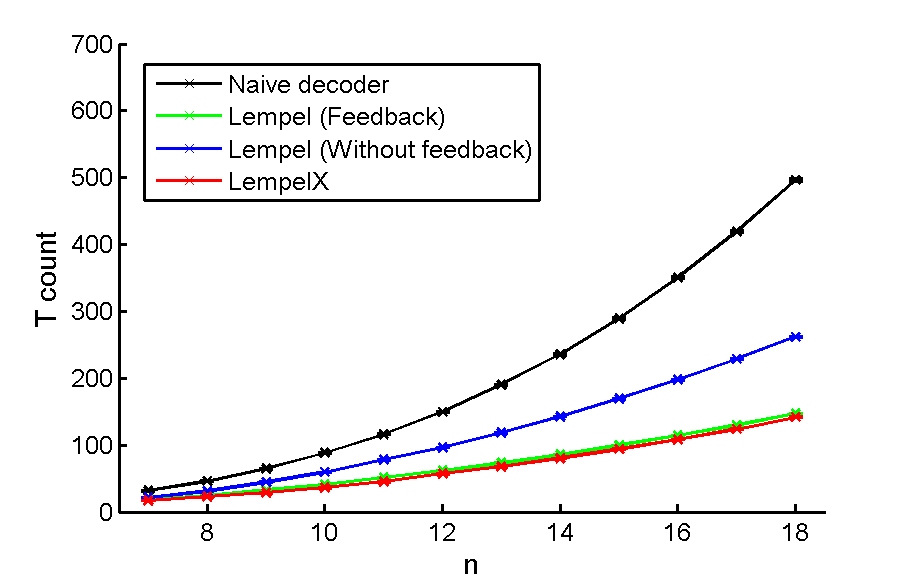
\includegraphics[width=\textwidth]{LX_vs_Lempel}
						\caption{}
						\label{f_random_a}
					\end{subfigure}
					\begin{subfigure}[h]{0.44\textwidth}
						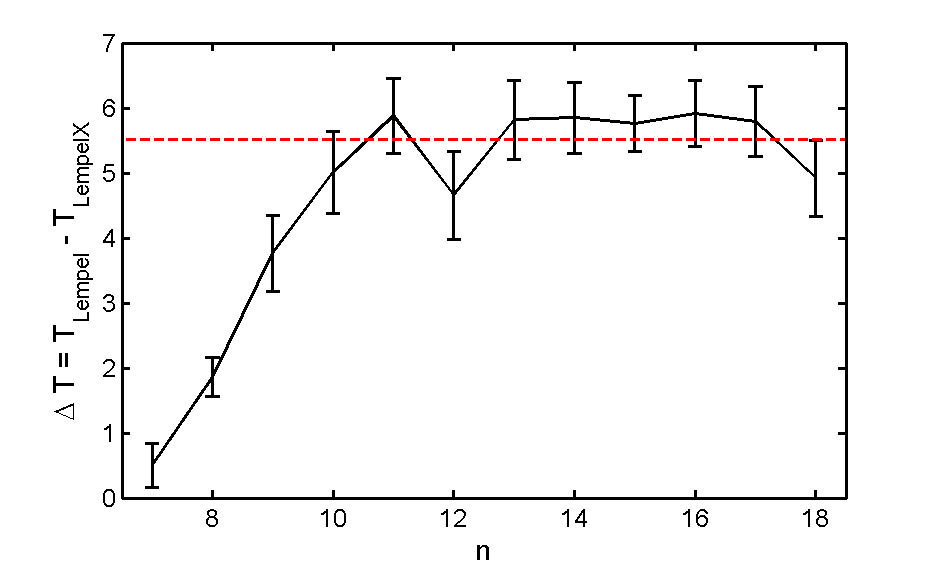
\includegraphics[width=\textwidth]{DeltaT}
						\caption{}
						\label{f_random_b}
					\end{subfigure}
					\caption{T counts for random circuits composed of CNOT and T gates synthesized by Lempel and LempelX.}
					\label{f_random}
				\end{figure}
				
				%\FloatBarrier
				\subsection{Universal Practical Circuits}
				The Lempel and LempelX algorithms were tested on universal circuits composed from CNOT, H and T gates and the results are compiled in table \ref{t_1}. These circuits were taken from Maslov's reversible benchmark website \cite{37_Maslov_web}. Multiply controlled Toffoli gates are constructed using a standard method demonstrated in figure \ref{f_toffn}. 
				Hadamards are eliminated using \ref{f_had}, which has the effect of swapping the Boolean variable associated with the qubit to which the Hadamard is applied with a completely new variable representing the ``Hadamard-ancilla''. This trick for Hadamard removal using so called \emph{path variables} is due to \cite{4_Amy_2013}. The addition of potentially hundreds of Hadamard-ancillas for large circuits could cause practical issues for the synthesis algorithms regarding time constraints.  A full investigation is yet to be conducted into the practical limits on space and time resources for our implementation of Lempel and LempelX. Until this is done, functionality has been included in our implementations to optionally divide the input circuit into partitions, each of which can only contain up to a specifiable maximum number of Hadamards.
				%Although the time and space resources for both Lempel and LempelX scale polynomial in $n$, the absolute time-scales for circuits with $n>100$ would probably not be practical.  phase polynomial by  Enforced a maximum Hadamard-ancilla count.
				% Toffoli-n
				\begin{figure}[h]
					\[
					\Qcircuit @C=1em @R=0.7em {
						& \ctrl{1} & \qw & \push{\rule{4em}{0em}} &  & \ctrl{1} & \qw & \ctrl{1} & \qw\\
						& \ctrl{1} & \qw & = &  & \ctrl{3} & \qw & \ctrl{3} & \qw\\
						& \ctrl{1} & \qw & &   &\qw & \ctrl{1} & \qw & \qw \\
						& \targ \qwx & \qw &  &  &\qw & \targ & \qw  & \qw\\
						&&&&\lstick{\ket{0}} & \targ \qwx & \ctrl{-1} & \targ & \qw
					}
					\]		
					\caption{Circuit showing a method to construct the the $4$-control Toffoli gate with standard Toffoli gates. The generalized $n$-controlled Toffoli can be constructed similarly with additional ancillas.}
					\label{f_toffn}
				\end{figure}
			
				% Removing Hadamards
				\begin{figure}[h]
					\[
					\Qcircuit @C=1em @R=1em {
						\lstick{\ket{\psi}} & \gate{H} &  \rstick{H\ket{\psi}}\qw & &\push{\rule{2em}{0em}=\rule{2em}{0em}} &  \lstick{\ket{\psi}} & \qw & \ctrl{1} & \qw & \qswap & \qw & \qw & \gate{X} & \rstick{H\ket{\psi}}\qw \\
						& & & & & \lstick{\ket{0}} & \gate{H} & \ctrl{-1} & \qw & \qswap \qwx & \qw & \gate{H} & \meter \cwx
					}
					\]
					\caption{Internal Hadamards are eliminated by delegating them to act on ancillas according to the above circuit identity. The Hadamards on the left-hand circuit are now external, therefore they no longer obstruct the Lempel and LempelX synthesis algorithms.}
					\label{f_had}
				\end{figure}
			
				\begin{table}
					\centering
					\caption{T counts for various benchmark circuits composed of CNOT, H and T gates as synthesized by the extended Lempel algorithm. $T_{\text{original}}$ are the results produced my Amy and Mosca in \cite{8_Amy_2016} and are listed for comparison. $N_H$ is the size of the ancilla registry for Hadamard-ancillas and $N_{\text{partitions}}$ is the number of partitions. All circuits are taken from \cite{37_Maslov_web}.}
					\label{t_1}
					\begin{tabularx}{0.9\linewidth}{ |X|r|r|r|r|r|r| }
						\hline						
						Circuit & $T_{\text{original}}\cite{8_Amy_2016}$ & $T_{\text{LempelX}}$ & $T_{\text{naive}}$ & $N_{partitions}$ & $N_{H}$ & Time (s) \\
						\hline						
						Cycle17\_3: & 1944 & 567 & 567 & 24 & 30 & 562.719 \\
						hwb6\_47\_107 & 71 & 55 & 102 & 1 & 36 & 91.713 \\
						hwb6-42-150 & 71 & 46 & 140 & 1 & 36 & 160.198 \\
						mod5d4 & 16 & 8 & 8 & 1 & 1 & 0.019 \\
						nth\_prime6\_inc\_55\_667 & 400 & 263 & 354 & 5 & 30 & 228.025 \\
						%nth\_prime8\_inc\_3346\_7618 & 3531 &  &  \\
						ham15-109-214 & 97 & 28 & 65 & 1 & 30 & 27.756 \\
						ham15-70 & 230 & 103 & 148 & 3 & 30 & 100.899 \\
						ham15tc1 & 1019 & 258 & 359 & 7 & 30 & 270.862 \\
						\hline
					\end{tabularx}					
				\end{table}
			%Circuit & T-count (Original) & T-count (LempelX) & T-count (Naive) & No. Partitions & No. Hadamards & Exec. Time (s) \\
			
			\FloatBarrier
			\section{Discussion, Conclusions and Plans for Future Work}
			\label{s6_Discussion}
			
			To summarize, in this report an algorithm was presented for reducing the T count of circuits over CNOT and T gates that extends the principle of Lempel's factoring algorithm to symmetric tensors of order 3. This was benchmark tested on randomized CNOT and T circuits and was found to perform marginally better than then next best algorithm. Finally, it was tested on universal circuits for which decompositions were found that use between $25\%$ and $77\%$ T gates compared to previous constructions from \cite{8_Amy_2016}. At this stage, how much of this decrease is attributable to the synthesis algorithm is unqualified, however it seems likely that it is mostly caused by discrepancies in other stages of circuit processing. For example, in this work path variables are used to effectively ``remove'' Hadamards but other methods exist for Hadamard avoidance such as breaking the circuit into partitions that alternate between columns of Hadamards and regions composed only of CNOT and T gates.
			
			There are many avenues for future work on T count optimization. Over the remaining two years of this project I plan to investigate the following:			
			\begin{itemize}
				\item The results for Lempel depend on the order that qubits are factorized and for LempelX, the order that columns pairs are searched. I wish to investigate whether there are any means of characterizing these variations in order to optimize both algorithms with respect to execution sequence.
				\item One avenue for improving T count optimization, especially for the universal construction, is to combine T count optimization algorithms with H count optimization such as in \cite{Abdessaied2014}. It seems intuitive that solutions to both problems would complement each other as Hadamards and T gates serve as mutual obstacles during gate synthesis.
				\item There may be other conditions for which columns of gate synthesis matrices can be eliminated. I wish to investigate this further.
				\item It is known that minimum distance decoding of $RM^*(n-4,n)$ is equivalent to determining the symmetric tensor rank of symmetric tensors of order 3. I will research the best available algorithms for performing this task.
				\item In its current form, LempelX does not use the optimal Reed-Muller decoder at any stage. I will modify LempelX in order to switch to the optimal decoder once the rank of the gate synthesis matrix is reduced to $\leq n_{RM}$ where $n_{RM}$ is the practical limit on the number of qubits for the Reed-Muller decoder.
			\end{itemize}
			
			
			%NOTE: 
			
			%NOTE: There may be other conditions that allow for the elimination of gate synthesis matrix columns.
			
			%NOTE: It is evident from our analysis of the gate synthesis problem in terms of gate synthesis matrix and signature tensors that the problem 
			
			%NOTE: Change effective no. qubits in Lempel algorithm to rank as matrix row operations on GF(2) are generated by CNOT operators. Therefore, more T gate savings may be available in cases where no. eff. qubits > rank.
			
			%NOTE: Could make a more expensive version of LempelX that uses the brute force decoder at the end - would require finding the rank of the gate synthesis matrix between every round of LempelXbase.
			
			%NOTE: Try another matrix extension featuring rows with the full expression in equation (Signature tensor). The more general matrix could flag more times when columns can be eliminated.
			
			\bibliographystyle{abbrv}
			\bibliography{keylit} % IMPORTANT! Remember to ammend arXiv references that have been published.
\end{document}